\section{\system Framework}
\label{sec:framework}

\subsection{\system Overview}

The central audit question in \system is whether a suspicious capability identified in an agentic skill is supported by sufficient evidence for a security finding. A skill may refer to a protected file, invoke a sensitive operation, or communicate with an external endpoint. Security assessment also requires evidence about how the relevant source, operation, and destination are related. \system organizes the analysis into three stages: capability screening, provenance construction, and security adjudication. Figure~\ref{fig:system-overview} presents the workflow.

\begin{figure*}[t]
    \centering
    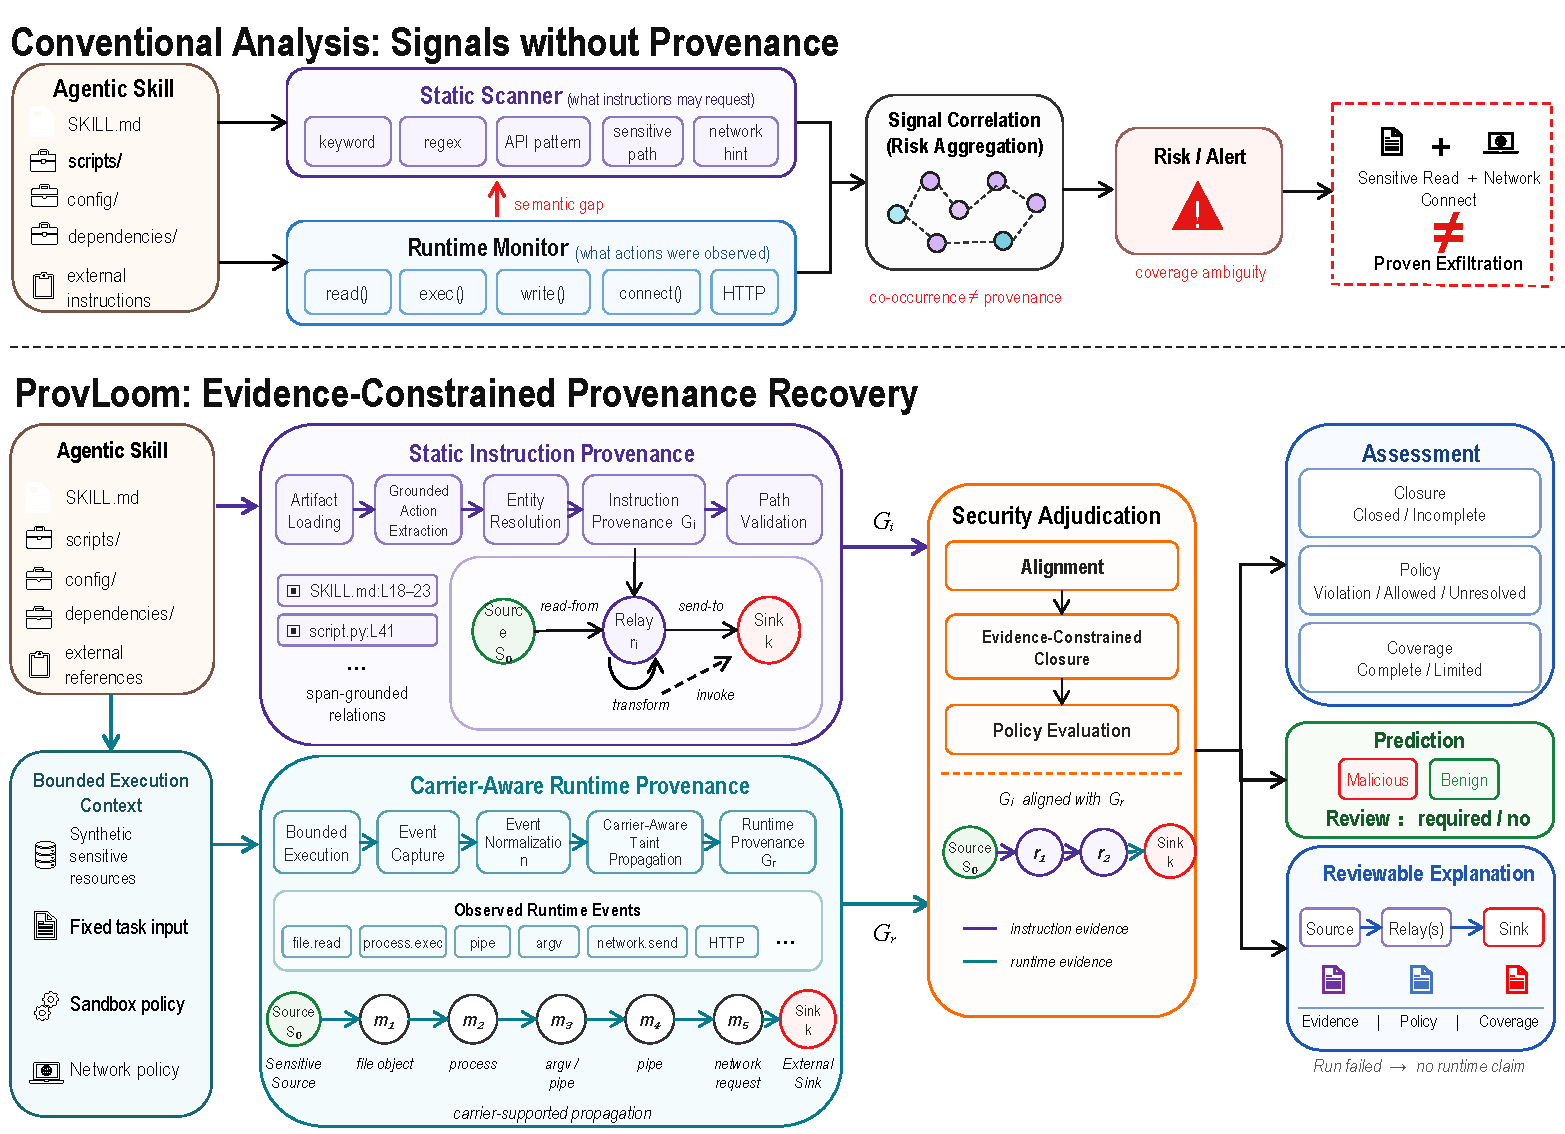
\includegraphics[width=\textwidth]{figures/fig1.pdf}
    \caption{Overview of the \system analysis workflow.}
    \label{fig:system-overview}
\end{figure*}

Capability screening starts from the skill bundle, including natural language instructions, helper scripts, package metadata, dependency declarations, and configuration files. Static analysis identifies security relevant operations and the entities involved in them. Instruction analysis lifts these observations into an instruction provenance graph. Typed entities and relations represent grounded sources, actions, destinations, modality, ordering constraints, and the instruction spans that support each relation. The resulting graph captures security relevant behavior expressed by the skill and provides candidate relations for subsequent analysis.

Provenance construction adds execution evidence through bounded replay. \system executes the skill in an instrumented environment and records file operations, process activity, tool interactions, LLM mediated actions, and network communication. Protected sources receive taint identities that propagate across LLM contexts, tool arguments and returns, files, processes, and network payloads. Runtime events and taint relations form a runtime provenance graph that records observed entities, operations, and data movement. Execution coverage is retained together with the runtime evidence.

The instruction and runtime graphs use compatible entity and relation types while preserving the origin of their evidence. Alignment associates compatible sources, actions, files, processes, endpoints, and other entities across the two graphs when their identifiers and semantics agree. An aligned relation records correspondence between stated behavior and an observed runtime event. Instruction evidence remains instruction evidence. Runtime confirmation requires observations produced during bounded execution.

Security adjudication operates over the aligned provenance representation. Closure analysis examines whether the available relations connect a protected source to a security relevant sink through supported carriers. A closed flow requires evidence that relates the source, intermediate data movement, and sink within the analyzed execution. Missing runtime realization, incomplete propagation, unavailable resources, and interrupted execution leave the corresponding path incomplete. Coverage records identify where the available execution evidence ends.

Policy analysis assigns security meaning to a supported flow. The policy decision considers the source, destination, operation, authorization context, and applicable trust assumptions. A supported flow may be classified as a violation, an authorized interaction, or an unresolved case when the available context is insufficient. Policy status is recorded separately from flow recovery so that an observed transfer does not determine its security status by itself.

The final assessment separates suspicious capability, observed flow, and policy violation. Each report records the security decision, supporting provenance path, relevant instruction spans, runtime evidence, policy status, and execution coverage. Incomplete paths retain the evidence recovered during analysis and the point at which stronger support could no longer be established.


\subsection{Threat Model}

\system considers third party agentic skills obtained from public repositories, marketplaces, or other untrusted distribution channels. An adversary may publish a malicious skill or modify an existing package before the skill reaches the user. The adversary controls natural language instructions, helper scripts, command templates, package metadata, dependency declarations, examples, configuration files, URLs, and setup or maintenance procedures. Malicious behavior may span several artifacts and may use generated files, tool calls, LLM mediated actions, process execution, data transformations, or network communication.

The adversary seeks to induce security relevant effects through ordinary skill execution. Confidentiality attacks may access protected data and transfer it to an unauthorized destination. Integrity attacks may execute untrusted code, modify protected state, establish persistence, or perform another unauthorized state change. Attack paths may depend on intermediate files, multiple processes, external services, conditional branches, delayed operations, or model selected actions.

The analysis environment controls the sandbox, instrumentation, synthetic protected resources, runtime policy, and controlled benchmark endpoints. The adversary cannot modify these trusted analysis components or directly compromise the underlying host. Real user credentials are excluded from the default audit environment. External services and platform state are available only when they are explicitly supplied by the execution context. Dynamic evidence is scoped to the task, environment, execution budget, and runtime interfaces observed during the corresponding replay.

The audit goal is to determine the strongest security claim supported by the available evidence. A confidentiality violation requires an observed information flow from a protected source to a destination prohibited by policy. An integrity violation requires evidence connecting skill driven behavior to the relevant protected operation or state change. Instruction provenance records security relevant behavior expressed by the package. Runtime provenance records behavior exercised during bounded execution. Alignment connects corresponding entities and relations while preserving the distinction between the two evidence sources.

Execution limits remain part of the assessment. Timeouts, unavailable environments, missing resources, untriggered branches, execution failures, external dependencies, and instrumentation gaps receive explicit coverage states. The report preserves the recovered evidence and the unresolved portion of the path for subsequent review.